\section{System Design}
\label{sec:design}

\sys realizes the overview design as a middleware/proxy around the agent's tool-dispatch path and LLM generation API, with scheduler hooks around the LLM serving engine.
This placement exposes the online event stream and per-session state used by three mechanisms: concrete prediction, interference-free speculative tool execution, and gain-preserving LLM-side pacing.

\subsection{Pattern Analyzer}
\label{sec:design-pattern-analyzer}

The Pattern Analyzer turns recurring agent-session structure into executable speculative invocation candidates.
The important point is that \sys does not only predict the next tool type; it predicts a concrete future invocation whose arguments can be derived from the current session history despite uncertainty in online agent execution.

\noindent\textbf{Event stream and representation.}
The event extractor records LLM turns, tool calls, tool outputs, timing signals, and session metadata from \sys's middleware/proxy event stream.
It normalizes each event into two parts: an event signature used for control-flow matching, and a payload retained for deriving concrete arguments.
Signatures intentionally capture stable control-flow information while excluding volatile natural-language content; payloads preserve the values that may later flow into predicted tool arguments.

\noindent\textbf{Prediction record.}
\sys stores each reusable prediction as a small pattern record.
The record contains a recent event context, a future tool target, an argument mapper, and an empirical confidence.
The context is matched over stable metadata such as tool type and success/failure status, while the mapper says where the future invocation's arguments should come from in the current session.

For example, after a successful search, a pattern may predict a web fetch and map its URL argument to the first URL in the current search result.
After a failed fetch, a fallback pattern can use the failure status and select the next URL from the same search result.
Thus the pattern captures recurring structure, while the live session supplies concrete values.

\noindent\textbf{Pattern pool construction.}
\sys builds the pattern pool in two passes.
First, it mines recurring short contexts over event signatures, which captures stable control flow while ignoring volatile natural-language payloads.
Second, it checks historical occurrences of each context to infer simple argument mappers, such as field lookup in structured tool output, choosing an indexed result with fallback, or lightweight string normalization.

Each candidate is validated against historical traces, and \sys keeps only patterns whose empirical probability is high enough for speculation.
Operator-supplied or offline-generated patterns can be added to the pool, but they pass through the same validation and confidence-estimation step before online use.

\noindent\textbf{Online prediction.}
For each live session, \sys maintains a bounded recent event window and matches the suffix of its signature stream against the validated pattern pool.
When a pattern matches, the analyzer applies the argument mapper to the current session's payloads.
This is late binding: the pattern decides what is likely to happen next, while the current session supplies the concrete values.
If the required payloads are already available, the analyzer emits a concrete invocation with tool name, canonicalized arguments, confidence, and expected latency benefit.
If only the tool identity or coarse parameters are known, the analyzer emits at most a preparation hint, not a fully executable tool call.
When multiple patterns match the same session state, the analyzer emits the corresponding hints without resolving conflicts locally; invocation-level arbitration is handled by the Tool Speculation Scheduler.
In both cases, prediction remains observational: the Pattern Analyzer forwards candidates to the Tool Speculation Scheduler and does not append anything to authoritative session state.

\subsection{Tool Speculation Scheduler}
\label{sec:design-tool-speculation-scheduler}

The Tool Speculation Scheduler moves concrete tool execution earlier in physical time while preserving the agent's semantic order.
Agent-issued tool calls enter the authoritative path exactly as before, while predicted calls enter a speculative path.
Both paths are launched through the same tool executor interface so that \sys can observe timing and reuse results, but speculative jobs and their outputs are isolated from authoritative session state until the LLM confirms the invocation.

\begin{figure}[t]
    \centering
    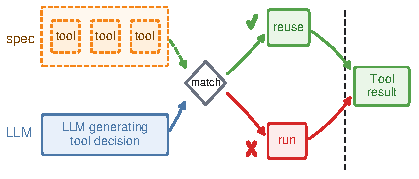
\includegraphics[width=0.88\linewidth]{images/ATC/speculative_tool_execution.pdf}
    \vspace{-0.2in}
    \caption{Lossless speculative tool execution.}
    \Description{Workflow showing speculative tool calls running in parallel with LLM generation, followed by a match decision that either reuses the speculative result or runs the authoritative tool call normally before committing a tool result.}
    \label{fig:spectool}
    \vspace{-0.2in}
\end{figure}

Figure~\ref{fig:spectool} illustrates the execution rule.
While the LLM is still generating its next tool decision, the scheduler may start one or more predicted tool calls in the speculative path.
When the LLM later emits the authoritative invocation, \sys compares the canonicalized tool name and arguments against speculative jobs.
On a hit, the completed result is reused, or an in-flight job is promoted into the authoritative path; on a miss, the invocation simply falls back to normal execution.
The commit boundary in the figure is crossed only by an authoritative invocation, either through reuse or through normal execution.
Thus speculation is lossless: a wrong prediction can waste bounded work, but it cannot expose an unconfirmed result to the agent, change the session history, or change the final state.

\noindent\textbf{Admission.}
Speculation is admitted by policy plus runtime conditions, not by blindly launching every prediction.
The scheduler first deduplicates predictions at the invocation level, so multiple matching patterns do not launch redundant work.

\noindent\textbf{Admission checks.}
A candidate is launched only if it passes four checks.
It must be executable, meaning the tool name and arguments are known and can be canonicalized for later matching.
It must be policy-safe, either because the tool is side-effect-free or because the deployment provides a safe speculative variant.
It must have enough confidence and expected exposed-tool-time benefit to justify the work.
Finally, the speculative budget must have room, so speculative work does not consume resources reserved for authoritative invocations.

\noindent\textbf{Speculation level and priority.}
Fully parameterized, side-effect-free tools may run end to end.
Partial predictions are limited to preparation work such as warm-up or dependency loading.
Tools with side effects require an explicit safe-speculation policy or a non-mutating transformed execution, such as dry-run execution or execution against staging resources; otherwise they are not speculated.
Among eligible candidates, \sys greedily favors higher expected utility per unit resource, combining prediction confidence, tool time likely to be hidden, resource demand, and expected duration.

\noindent\textbf{Non-interference.}
Authoritative invocations keep the normal tool scheduling policy and priority.
Speculative jobs run only within bounded or opportunistic capacity, are lower priority, and can be suppressed or preempted when authoritative work needs resources.
When contention forces preemption, \sys reclaims speculative work before authoritative work and chooses lower-utility speculative jobs first.
This resource rule keeps speculative execution from delaying correctness-critical tool work across concurrent sessions, while the state-isolation rule keeps speculation from changing the agent-visible history before confirmation.

\noindent\textbf{Match and promotion.}
When an authoritative invocation arrives, \sys compares its tool name and arguments with completed and in-flight speculative jobs.
A completed match is reused directly.
An in-flight match is promoted to authoritative execution and becomes non-preemptible.
If no match exists, the authoritative invocation runs normally through the tool executor.

\noindent\textbf{Misses and signals.}
Every speculative job has one of four outcomes.
It is reused if it has completed and later matches an authoritative invocation, promoted if it is still running when the match arrives, discarded if no match arrives before expiry, or preempted if authoritative work needs the resources.
Only the first two outcomes can commit a result to authoritative session state.

The scheduler reports normal completions, reused results, promoted jobs, discarded jobs, preemptions, and the amount of exposed tool time saved to the LLM--Tool Co-Scheduler, which uses these cross-domain signals for LLM-side pacing.

\subsection{LLM--Tool Co-Scheduler}
\label{sec:design-llm-tool-coscheduler}

The LLM--Tool Co-Scheduler converts local tool overlap into task-level end-to-end latency reduction.
It is a separate scheduler from the Tool Speculation Scheduler: it consumes tool-side signals, but its decision point is LLM-side pacing.
Its central rule is to admit the ready LLM turn that preserves the largest expected exposed-tool-time reduction per unit of current LLM pressure.
This preserves tool-side gains while keeping the LLM engine in its task-optimal load region, instead of admitting every returned session as soon as its tool finishes.

\begin{figure}[t]
\centering
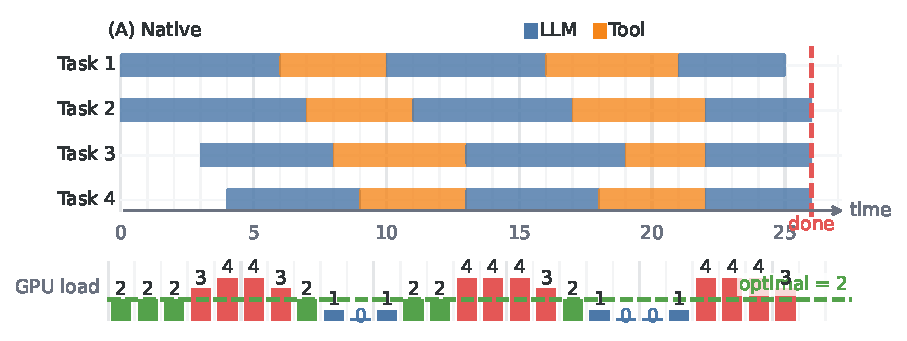
\includegraphics[width=\linewidth]{images/ATC/agent_aware_overlap_duration_matched_4tasks_left.pdf}
\vspace{-0.05in}
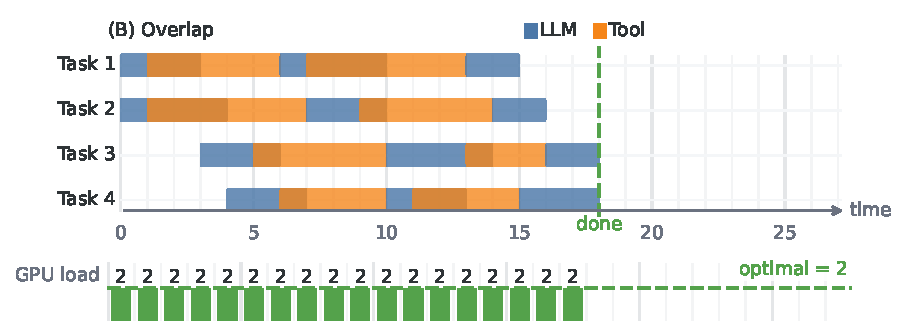
\includegraphics[width=\linewidth]{images/ATC/agent_aware_overlap_duration_matched_4tasks_right.pdf}
\caption{Gain-preserving LLM--tool co-scheduling keeps LLM load near the task-optimal region.}
\Description{Two timeline panels compare native execution and overlapped execution for four tasks. Native execution finishes later and shows LLM GPU load fluctuating above and below the optimal load, while overlapped execution finishes earlier and keeps GPU load close to the optimal level.}
\vspace{-0.2in}
\label{fig:cosched-example}
\end{figure}

Figure~\ref{fig:cosched-example} makes the source of the gain concrete.
In the native schedule, each task alternates between LLM and tool phases independently, so aggregate LLM load repeatedly overshoots the optimal region and then drops into under-utilized gaps.
Shortening a tool wait alone would not necessarily reduce task latency, because the saved time can be converted into extra LLM queueing or slower decoding when many sessions return together.
In the co-scheduled timeline, tool waits are hidden behind useful LLM work from other sessions, and returning sessions are admitted only fast enough to keep the GPU near the task-optimal load.
The completion boundary therefore moves earlier not because an individual LLM or tool operation becomes faster, but because exposed tool time is removed without creating a compensating LLM-side bottleneck.

\noindent\textbf{Inputs and state.}
The co-scheduler consumes tool-side completion signals from authoritative execution, completed speculative jobs, and promoted in-flight speculative jobs.
These signals reveal how much exposed tool time has already been reduced and which sessions risk losing that gain to LLM queueing.
\sys also tracks each session's position in the LLM--tool chain: whether it is a new cold session, an active foreground session, a session returning from a tool, or a session likely to expose another tool wait after its next LLM turn.
For each ready turn, \sys estimates exposed-tool-time gain from recent service times, observed tool waits, pattern-derived next-tool likelihood, and session progress, while also tracking current LLM pressure.

\noindent\textbf{Pre-engine admission.}
The first control point is a pre-engine admission queue that decides which ready LLM turns are released into the serving engine.
The scheduler releases ready work to avoid GPU idle time when running concurrency is low, and softly gates new cold sessions once the engine has enough running work so the system does not spread capacity across too many partial sessions.
Among eligible turns, \sys ranks by gain efficiency:
\[
\mathrm{priority}(i) =
    \frac{\mathrm{ExposedToolGain}(i)}
         {\mathrm{LLMPressure}(i,\mathrm{load})}
    + \mathrm{Aging}(i).
\]
\texttt{ExposedToolGain} is the expected reduction in task-critical exposed tool time from admitting the turn now.
It has two concrete sources: realized gain from a completed or promoted tool result that can be consumed immediately, and future gain from reaching the next predictable tool wait early enough for speculation to hide it.
\texttt{LLMPressure} is the incremental pressure of admitting the turn now, including predicted LLM service time, current queue and batch pressure, context length, and KV/cache pressure.
\texttt{Aging} is a small fairness term.
Returned or promoted sessions are therefore not released merely because their tools finished; they are released when doing so preserves expected exposed-tool-time gain at acceptable LLM pressure.

\noindent\textbf{In-engine load shaping.}
The second control point is an in-engine load-shaping hook that keeps the running batch within the task-optimal load region after turns have been admitted.
The scheduler observes active requests, decode batch pressure, queue depth, context length distribution, and KV/cache pressure, and feeds these measurements back to update \texttt{LLMPressure}.
\sys summarizes the running batch with an engine-pressure score:
\[
\mathrm{EnginePressure}(B) =
    \mathrm{DecodeLoad}(B) + \gamma \cdot \mathrm{KVLoad}(B),
\]
\sys then keeps this score within a workload-aware pressure band:
\[
P_{\mathrm{low}} \le \mathrm{EnginePressure}(B) \le P_{\mathrm{high}}.
\]
Here $B$ is the current active or admitted batch; \texttt{DecodeLoad} captures active decoding work, while \texttt{KVLoad} summarizes context and KV-cache pressure.
This load shaping keeps the engine away from both under-utilization and overload, while preserving the serving engine's normal token-level scheduling inside the admitted set.
Together, pre-engine pacing and in-engine load shaping maximize preserved exposed-tool-time reduction under LLM load constraints, reducing partial-session work and avoiding the conversion of saved tool time into extra LLM queueing or decoding time.
